\RequirePackage{currfile}
\documentclass[12pt]{beamer}
\usepackage[utf8]{inputenc}
\usepackage[spanish]{babel}
\usepackage{standalone}
\usepackage{color}
\usepackage{siunitx}
\usepackage{hyperref}
%\hypersetup{colorlinks,linkcolor=,urlcolor=blue}
%\hypersetup{colorlinks,urlcolor=blue}
\usepackage{xcolor,soul}
\usepackage{etoolbox}
\usepackage{amsmath}
\usepackage{amsthm}
\usepackage{physics}
\usepackage{multicol}
\usepackage{bookmark}
\usepackage{longtable}
\usepackage{listings}
\usepackage{graphicx}
\usepackage{tikz}
\usetikzlibrary{patterns, matrix, backgrounds, decorations,shapes, arrows.meta}
\usepackage[autostyle,spanish=mexican]{csquotes}
\usepackage[os=win]{menukeys}
\usepackage{pifont}
\usepackage{pbox}
\usepackage{caption}
\captionsetup{font=scriptsize,labelfont=scriptsize}
%\usepackage[sfdefault]{roboto}  %% Option 'sfdefault' only if the base font of the document is to be sans serif

%Sección de definición de colores
\definecolor{ao}{rgb}{0.0, 0.5, 0.0}
\definecolor{bisque}{rgb}{1.0, 0.89, 0.77}
\definecolor{amber}{rgb}{1.0, 0.75, 0.0}
\definecolor{armygreen}{rgb}{0.29, 0.33, 0.13}
\definecolor{alizarin}{rgb}{0.82, 0.1, 0.26}
\definecolor{cadetblue}{rgb}{0.37, 0.62, 0.63}
\definecolor{deepblue}{rgb}{0,0,0.5}
\definecolor{brown}{rgb}{0.59, 0.29, 0.0}
\definecolor{OliveGreen}{rgb}{0,0.25,0}


\usefonttheme[onlymath]{serif}
%Sección de definición de nuevos comandos

\newcommand*{\TitleParbox}[1]{\parbox[c]{1.75cm}{\raggedright #1}}%
\newcommand{\python}{\texttt{python}}
\newcommand{\textoazul}[1]{\textcolor{blue}{#1}}
\newcommand{\azulfuerte}[1]{\textcolor{blue}{\textbf{#1}}}
\newcommand{\funcionazul}[1]{\textcolor{blue}{\textbf{\texttt{#1}}}}
\newcommand{\ptilde}[1]{\ensuremath{{#1}^{\prime}}}
\newcommand{\stilde}[1]{\ensuremath{{#1}^{\prime \prime}}}
\newcommand{\ttilde}[1]{\ensuremath{{#1}^{\prime \prime \prime}}}
\newcommand{\ntilde}[2]{\ensuremath{{#1}^{(#2)}}}
\renewcommand{\arraystretch}{1.5}

\newcounter{saveenumi}
\newcommand{\seti}{\setcounter{saveenumi}{\value{enumi}}}
\newcommand{\conti}{\setcounter{enumi}{\value{saveenumi}}}
\renewcommand{\rmdefault}{cmr}% cmr = Computer Modern Roman

\linespread{1.5}

\usefonttheme{professionalfonts}
%\usefonttheme{serif}
\DeclareGraphicsExtensions{.pdf,.png,.jpg}


%Sección para el tema de beamer, con el theme, usercolortheme y sección de footers
\mode<presentation>
{
  \usetheme{Warsaw}
  
  %\useoutertheme{infolines}
  \useoutertheme{default}
  \usecolortheme{spruce}
  \setbeamercovered{invisible}
  % or whatever (possibly just delete it)
  \setbeamertemplate{section in toc}[sections numbered]
  \setbeamertemplate{subsection in toc}[subsections numbered]
  \setbeamertemplate{subsection in toc}{\leavevmode\leftskip=3.2em\rlap{\hskip-2em\inserttocsectionnumber.\inserttocsubsectionnumber}\inserttocsubsection\par}
  \setbeamercolor{section in toc}{fg=blue}
  \setbeamercolor{subsection in toc}{fg=blue}
  \setbeamercolor{frametitle}{fg=blue}
  \setbeamertemplate{caption}[numbered]

  \setbeamertemplate{footline}
  \beamertemplatenavigationsymbolsempty
  \setbeamertemplate{headline}{}
}

\makeatletter
\setbeamercolor{section in foot}{bg=gray!30, fg=black!90!orange}
\setbeamercolor{subsection in foot}{bg=blue!30!yellow, fg=red}
\setbeamertemplate{footline}
{
  \leavevmode%
  \hbox{%
  \begin{beamercolorbox}[wd=.333333\paperwidth,ht=2.25ex,dp=1ex,center]{section in foot}%
    \usebeamerfont{section in foot} \insertsection
  \end{beamercolorbox}}%
  \begin{beamercolorbox}[wd=.333333\paperwidth,ht=2.25ex,dp=1ex,center]{subsection in foot}%
    \usebeamerfont{subsection in foot}  \insertsubsection
  \end{beamercolorbox}%
  \begin{beamercolorbox}[wd=.333333\paperwidth,ht=2.25ex,dp=1ex,right]{date in head/foot}%
    \usebeamerfont{date in head/foot} \insertshortdate{} \hspace*{2em}
    \insertframenumber{} / \inserttotalframenumber \hspace*{2ex} 
  \end{beamercolorbox}}%
  \vskip0pt%
\makeatother  

\makeatletter
\patchcmd{\beamer@sectionintoc}
  {\vfill}
  {\vskip\itemsep}
  {}
  {}
\makeatother


\newcommand{\Cancel}[2][black]{{\color{#1}\cancel{\color{black}#2}}}
\title{\large{Asesoría Repaso Tema 1}}
\author{M. en C. Gustavo Contreras Mayén}
\date{\today}
\institute{Facultad de Ciencias - UNAM}
\titlegraphic{
\includegraphics[width=1.75cm]{../Imagenes/escudo-facultad-ciencias}\hspace*{4.75cm}~%
   
\includegraphics[width=1.75cm]{../Imagenes/escudo-unam}
}
\setbeamertemplate{navigation symbols}{}
\begin{document}
\maketitle
\fontsize{14}{14}\selectfont
\spanishdecimal{.}
\section*{Contenido}
\frame{\tableofcontents[currentsection, hideallsubsections]}

\section{Funciones Gamma y Beta}
\frame{\tableofcontents[currentsection, hideothersubsections]}
\subsection{Repaso de las funciones}

\begin{frame}
\frametitle{Las funciones Gamma y Beta}
En la parte del curso en donde trabajamos con las funciones Gamma y Beta, se presentó la definición de cada una de ellas en términos de una integral:
\end{frame}
\begin{frame}
\frametitle{Función Gamma}
La función Gamma para cualquier $p >0$, es:
\begin{align*}
\Gamma (p) = \int_{0}^{\infty} x^{p-1} \, e^{-x} \dd{x}, \hspace{1cm} p > 0
\end{align*}
\pause
Mientras que la función Beta: 
\begin{align*}
\begin{gathered}
B(p, q) = \int_{0}^{1} x^{p-1} \, (1- x )^{q-1} \dd{x}, \\
\mbox{con }  p > 0, q > 0
\end{gathered}
\end{align*}
\end{frame}
\begin{frame}
\frametitle{Propiedades de las funciones}
Posteriormente se revisaron algunas de las propiedades tanto para la función Gamma como para la función Beta, se realizó la demostración de esas propiedades (no todas), a partir de la definición de las funciones.
\end{frame}
\begin{frame}
\frametitle{Relación entre la función Gamma y Beta}
Se revisó también una relación entre la función Beta y Gamma, que nos permite entonces obtener un valor ya sea en términos de factores de $\sqrt{\pi}$ o en su caso, un valor númerico.
\end{frame}
\begin{frame}
\frametitle{Utilidad de las funciones}
En física encontraremos estas funciones en desarrollos que involucran el manejo de los factoriales, es por ello que nos conviene su uso.
\\
\bigskip
\pause
También serán de utilidad para resolver algunas integrales que en apariencia son complicadas, aprovechando las propiedades de ambas funciones.
\end{frame}

\section{Resolviendo integrales}
\frame{\tableofcontents[currentsection, hideothersubsections]}
\subsection{Ejercicio 1}

\begin{frame}
\frametitle{Ejercicio 1-  Enunciado}
Calcula el área $A$ encerrada entre el eje $x$ y un arco de la curva $y = \sin^{8} x$ en el intervalo $[0, \pi]$.
\end{frame}
\begin{frame}
\frametitle{Planteamiento del ejercicio}
Lo que se nos pide es calcular el área debajo de la curva que se muestra a continuación:
\begin{figure}
    \centering
    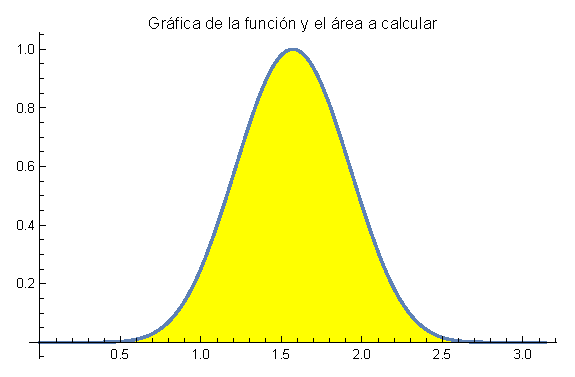
\includegraphics[scale=0.9]{Imagenes/Asesoria_03_01.eps}
\end{figure}
\end{frame}
\begin{frame}
\frametitle{Planteamiento del problema}
Sabemos por el curso de Cálculo II, que el área debajo de la curva la podemos obtener resolviendo la integral:
\begin{align*}
A = \int_{0}^{\pi} \sin^{8} x \dd{x}
\end{align*}
\pause
De entrada la integral no se mira amigable como para usar alguna identidad trigonométrica o algún cambio de variable tan inmediato.
\end{frame}
\begin{frame}
\frametitle{Antes de ocupar una expresión}
Con la finalidad de simplificar la expresión, vemos de la gráfica anterior, que podemos calcular la integral (y por lo tanto, conocer el área $A$), al reducir el intervalo de integración, aprovechando la simetría de la curva:
\begin{align*}
A = 2 \int_{0}^{\frac{\pi}{2}} \sin^{8} x \dd{x}
\end{align*}
\end{frame}
\begin{frame}
\frametitle{Aprovechamos una identidad de $B(x,y)$}
El integrando de interés lo podemos multiplicar por un $1$ en particular: $\cos^{0} x$, de tal manera que quede expresado como:
\begin{align*}
A = 2 \int_{0}^{\frac{\pi}{2}} \sin^{8} x \cos^{0} x \dd{x}
\end{align*}
\pause
que podemos dejar como:
\begin{align*}
A = \int_{0}^{\frac{\pi}{2}} 2 \, \sin^{8} x \cos^{0} x \dd{x}
\end{align*}
\end{frame}
\begin{frame}
\frametitle{Cambio de variable}
Si hacemos el cambio de variable $x = \theta$, llegamos a:
\begin{align*}
A = \int_{0}^{\frac{\pi}{2}} 2 \, \sin^{8} \theta \cos^{0} \theta \dd{\theta}
\end{align*}
\pause
Por lo que podemos usar la identidad:
\begin{align*}
B(x, y) = \int_{0}^\frac{\pi}{2} 2 \, \sin^{2x-1} \theta \, \cos^{2y-1} \theta \dd{\theta}
\end{align*}
\end{frame}
\begin{frame}
\frametitle{Usando la identidad}
Entonces tendremos que:
\begin{align*}
2 \, x - 1 = 8 &\Rightarrow x = \dfrac{9}{2} \\[0.5em]
2 \, y - 1 = 0 &\Rightarrow y = \dfrac{1}{2}
\end{align*}
\pause
Por lo que la integral pasa a ser:
\begin{align*}
A = B \left( \dfrac{9}{2},\dfrac{1}{2} \right)
\end{align*}
\end{frame}
\begin{frame}
\frametitle{Recuperando el valor del área}
Nos queda entonces obtener el valor de la función Beta con los argumentos dados, y tendremos entonces el valor del área solicitado.
\\
\bigskip
\pause
Ocuparemos una relación entre las funciones Gamma y Beta, y entonces evaluar la función Gamma para obtener dicho valor del área.
\end{frame}
\begin{frame}
\frametitle{Relación función Beta y Gamma}
Sabemos que:
\begin{align*}
B (x, y) = \dfrac{\Gamma (x) \, \Gamma (y)}{\Gamma (x + y)}
\end{align*}
\pause
Entonces:
\begin{align*}
A &= B \left( \dfrac{9}{2},\dfrac{1}{2} \right) = \dfrac{\Gamma \left(\dfrac{9}{2} \right) \, \Gamma \left(\dfrac{1}{2} \right)}{\Gamma \left(\dfrac{9}{2} + \dfrac{1}{2} \right)}
\end{align*}
\end{frame}
\begin{frame}
\frametitle{Calculando los valores de $\Gamma(x)$}
Obtenemos los valores de la función Gamma:
\begin{eqnarray*}
\Gamma \left( \dfrac{1}{2} \right) &=& \sqrt{\pi} \\[0.5em] \pause
\Gamma \left( \dfrac{9}{2} + \dfrac{1}{2} \right) &=& \Gamma (5) = (5 - 1)! = 4! = 24 \\[0.5em] \pause
\Gamma \left(n + \dfrac{1}{2}\right) &=& \dfrac{1 \cdot 3 \cdot 5 \ldots (2 \, n - 1)}{2^{n}} \, \sqrt{\pi} 
\end{eqnarray*}
\end{frame}
\begin{frame}
\frametitle{Calculando los valores para $\Gamma (x)$}
Para el último valor, se tiene que:
\begin{align*}
\Gamma \left( \dfrac{9}{2}\right) &=  \Gamma \left(4 + \dfrac{1}{2}\right) = \dfrac{1 \cdot 3 \cdot 5 \cdot (2 \cdot 4 - 1)}{2^{4}} \, \sqrt{\pi} \\[1em]
&= \dfrac{105 \sqrt{\pi}}{16}
\end{align*}
\end{frame}
\begin{frame}
\frametitle{El valor del área $A$}
Tendremos entonces que el valor del área es:
\begin{align*}
A &= \dfrac{\dfrac{105 \sqrt{\pi}}{16} \, \sqrt{\pi}}{24} = \\[0.5em]
&= \dfrac{105 \sqrt{\pi}}{384} = \\[0.5em]
&= \dfrac{35 \, \pi}{128} \qed
\end{align*}
\end{frame}

\subsection{Ejercicio 2}

\begin{frame}
\frametitle{Planteamiento del ejercicio}
Calcula el área $A$ encerrada en el óvalo definido por:
\begin{align*}
y^{2} = \dfrac{1 - x^{2}}{1 + x^{2}}
\end{align*}
\end{frame}
\begin{frame}
\frametitle{Explorando previamente el enunciado}
Un paso que se recomienda siempre, es el de contar con una referencia gráfica de la función que se nos presenta.
\\
\bigskip
\pause
Para ello ocupamos cualquier programa que nos genere la gráfica:
\end{frame}
\begin{frame}
\frametitle{Gráfica de la función}
Tenemos la gráfica:
\begin{figure}
    \centering
    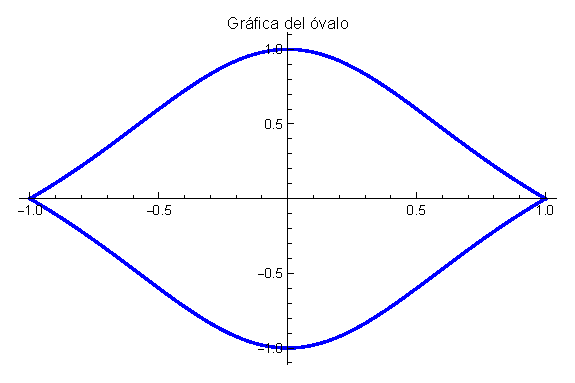
\includegraphics[scale=1]{Imagenes/Asesoria_03_02.eps}
\end{figure}
\end{frame}
\begin{frame}
\frametitle{Revisando la gráfica}
Observamos que esta curva está limitada por las líneas $x \pm 1$, ya que $y^{2}$ sería negativo para $\abs{x} > 1$.
\\
\bigskip
\pause
De manera similar, al resolver para $x^{2}$, se encuentra que la curva está limitada por las líneas $y = \pm 1$. La restricción sobre $x$ sugiere un cambio de variable.
\end{frame}
\begin{frame}
\frametitle{Cambio de variable}
Sea el cambio de variable:
\begin{align*}
x^{2} = \sin t \hspace{0.2cm} \Rightarrow \hspace{0.2cm} \dd{x} = \dfrac{1}{2} \dfrac{\cos t}{\sqrt{\sin t}} \dd{t}
\end{align*}
\pause
Adicionalmente tenemos que la curva es simétrica en ambos ejer coordenados, por lo que podemos calcular el área en el primer cuadrante y multiplicar por $4$ para obtener el área total.
\end{frame}
\begin{frame}
\frametitle{Cuadrante del óvalo}
\begin{figure}
    \centering
    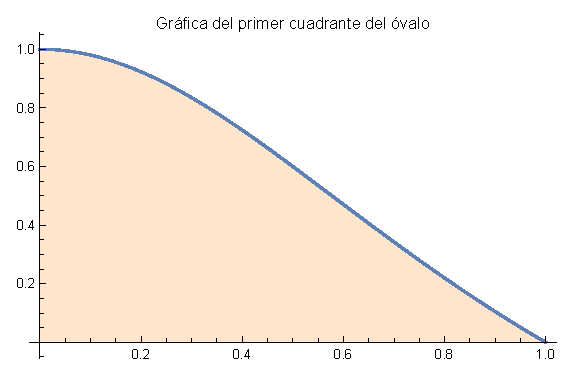
\includegraphics[scale=1]{Imagenes/Asesoria_03_03.eps}
\end{figure}
\end{frame}
\begin{frame}
\frametitle{Resolviendo el problema}
Tenemos entonces que:
\begin{align*}
A = 4 \int_{0}^{1} y \dd{x} =  4 \int_{0}^{\frac{\pi}{2}} \sqrt{{\dfrac{1 - \sin t}{1 + \sin t}}} \, \cdot \dfrac{1}{2} \, \dfrac{\cos t}{\sqrt{\sin t}} \dd{t}
\end{align*}
\pause
Que nuevamente aparenta complicar más el integrando, pero recurrimos al álgebra para intentar simplificarlo:
\end{frame}
\begin{frame}
\frametitle{Manejo algebraico}
Si multiplicamos el radical del integrando por un $1 = 1 - \sin t / 1 \sin t$, tendremos:
\begin{eqnarray*}
A &=& 2 \int_{0}^{\frac{2}{\pi}} \sqrt{\dfrac{(1 - \sin t)^{2}}{\cos^{2} t}} \, \dfrac{\cos t}{\sqrt{\sin t}} \dd{t} = \\[1em]
&=& 2 \int_{0}^{\frac{\pi}{2}} \big( \sin^{-\frac{1}{2}} t - \sin^{\frac{t}{2}} t \big) \dd{t} = \\[1em]
&=& 2 \int_{0}^{\frac{\pi}{2}} \dfrac{\dd{t}}{\sin^{\frac{1}{2} t}} - 2 \int_{0}^{\frac{\pi}{2}} \sin^{\frac{1}{2}} t \dd{t}
\end{eqnarray*}
\end{frame}
\begin{frame}
\frametitle{Sobre las integrales obtenidas}
\begin{align*}
A = 2 \int_{0}^{\frac{\pi}{2}} \dfrac{\dd{t}}{\sin^{\frac{1}{2} t}} - 2 \int_{0}^{\frac{\pi}{2}} \sin^{\frac{1}{2}} t \dd{t}
\end{align*}
La segunda de estas dos integrales es propia, pero la primera es impropia.
\end{frame}
\begin{frame}
\frametitle{Sobre las integrales obtenidas}
Sabemos que \emph{la integral impropia debe ser convergente} porque sabemos que el área $A$ es finita, ya que $A$ está completamente contenida dentro de un cuadrado de lado 2.
\\
\bigskip
\pause
Veamos la convergencia de la integral impropia.
\end{frame}
\begin{frame}
\frametitle{Estudiando la integral}
La razón $t/\sin t \to 1$ cuando en el límite $t \to 0$.
\\
\bigskip
\pause
Esto hace que el integrando sea \enquote{similar} a $1 / t^{1/2}$ mientras $t \to 0$, con la consecuencia de que la convergencia de la integral
\begin{align*}
\int_{0}^{\frac{\pi}{2}} \dfrac{\dd{t}}{\sin^{\frac{1}{2} t}}
\end{align*}
depende ya sea de la convergencia o divergencia de:
\begin{align*}
\int_{0}^{\frac{\pi}{2}} \dfrac{\dd{t}}{t^{\frac{1}{2}}}
\end{align*}
\end{frame}
\begin{frame}
\frametitle{Estudiando la integral}
\begin{align*}
\int_{0}^{\frac{\pi}{2}} \dfrac{\dd{t}}{t^{\frac{1}{2}}}
\end{align*}
Pero sabemos que esta última integral es convergente porque el exponente en $t$ es menor que la unidad.
\\
\bigskip
\pause
Por tanto, la integral en cuestión también es convergente.
\end{frame}
\begin{frame}
\frametitle{Completando la integral}
Ahora insertamos el factor $\cos^{0} t$ que nos permite reconocer las integrales como integrales Beta:
\begin{align*}
A = \int_{0}^{\frac{\pi}{2}} 2 \sin^{-\frac{1}{2}} t \cos^{0} t \dd{t} - \int_{0}^{\frac{\pi}{2}} 2 \sin^{\frac{1}{2}} t \cos^{0} t \dd{t}
\end{align*}
\pause
Por la identidad anteriormente utilizada:
\begin{align*}
A = B \left( \dfrac{1}{4}, \dfrac{1}{2} \right) - B \left( \dfrac{3}{4}, \dfrac{1}{2} \right)
\end{align*}
\end{frame}
\begin{frame}
\frametitle{Expresión a evaluar}
Tenemos entonces que calcular:
\begin{align*}
A = \dfrac{\sqrt{\pi} \, \Gamma \left( \dfrac{1}{4} \right)}{\Gamma \left( \dfrac{3}{4} \right)} - \dfrac{\sqrt{\pi} \, \Gamma \left( \dfrac{3}{4} \right)}{\Gamma \left( \dfrac{5}{4} \right)}
\end{align*}
\end{frame}
\begin{frame}
\frametitle{Resultado}
Haciendo las respectivas operaciones para evaluar las funciones Gamma con los argumentos, y simplificando con un valor numérico (que se puede obtener mediante el uso de software matemático o de programación), tenemos que el área $A$ en cerrada en el óvalo inicial es:
\pause
\begin{align*}
A = 2.847
\end{align*}
\end{frame}
\end{document}